\chapter{Benders decomposition}
\label{chap:benders}

\section{Introduction}

Benders decomposition is a solution method for solving certain large-scale optimization problems. It is particularly suited for problems in which a set of variables are said to be \textit{complicating} in the sense that fixing them to a given value makes the problem easy. Briefly, the Benders decomposition approach seperates an original problem into several decision stages. A first-stage \textit{master} problem is solved using only a subset of variables, then, the values of the remaining variables are determined by a so-called \textit{subproblem} depending on the first-stage variables. If the master problem's optimal solution yields an infeasible subproblem, a \textit{feasibility cut} is added to the master problem, which is then re-solved. Due to the structure of the reformulation, the Benders algorithm starts with a \textit{restricted master problem} where only a subset of constraints are considered while the others are iteratively added. 

This technique was first introduced in \cite{Benders1962} and has since been generalized to non-linear mixed integer problems. 

\section{Formal derivation}

Consider the following problem :
\begin{align}
    \textrm{minimize } & c^Tx + f(y) \\
    \textrm{s.t. } & Ax + g(y) = b \\
    & y\in Y, x\ge 0
\end{align} where variable $y$ is a \textit{complicating constraint}. Note that it may be complicating due to the form of $f$ or $g$ but also by our ability to enforce the constraint $y\in Y$. We assume that fixing $y$ to a given value $\hat y$ turns our problem into an easy-to-solve problem. 

We can notice that our problem is equivalent to the following one : \[
    \min\left\{ f(y) + \min\left\{ c^Tx : Ax = b - g(y) \right\} : y \in Y \right\}
\] Let us denote by $q(y)$ the value of the minimization problem over $x$ : $q(y) = \min\{ c^Tx : Ax = b - g(y) \}$. By duality, the following holds \[
    q(y) = \max\{ (b-g(y))^T\pi : A^T\pi \le c \}
\] Note that the feasibility space of the dual does not depend on the values of $y$ and let us apply the decomposition theorem for polyhedra \ref{th:decomposition_polyhedra} on it :
\begin{align*}
    &\{ A^T\pi \le c \} = \left\{ \sum_i u^i\alpha_i + \sum_j v^j\beta_j \right\} \\
    &\sum_i \alpha_i = 1 \quad\textrm{and}\quad \alpha, \beta \ge 0
\end{align*} where $\{u^i\}_i$ denotes the extreme points of $\{x|Ax\le c\}$ and $\{v^j\}_j$ denotes the extreme rays of the polyhedral cone $\{x|Ax\le 0\}$. Intuitively, the convex combination of the extreme points of $\{x|Ax\le c\}$ defines the optimal solutions (since we know that there exists at least one optimal solution corresponding to an extreme point of the considered polyhedron) while the conical combination of extreme rays of $\{x|Ax\le 0\}$ defines the feasibility region. The following theorem will allow us to reformulate our problem :
\begin{theorem}
    \label{th:upper_bounded_problem_theorem}
    Let ($\mathcal P$) be the following problem : \[ \max\{ c^Tx : Ax \le b, x\ge 0 \} \tag{$\mathcal P$} \] Then, ($\mathcal P$) is upper bounded if and only if 
    \[ c^Tv^j \le 0\quad \forall j=1,...,J \]
    where $\{v^j\}_{j=1,...,J}$ denotes the set of extreme rays of $\{x|Ax\le 0\}$. 
\end{theorem}
\begin{proof}
$\Rightarrow$ : By contradiction, let us suppose that $(\mathcal P)$ is upper bounded and that there exists $k$ such that $c^Tv^k > 0$. Let us consider a feasible solution to ($\mathcal P$) denoted by $u = z + t$ where $z$ is a convex combination of the extreme points of $\{x|Ax\le b\}$ and $t$ an element of the conical combinations of the extreme rays of $\{x|Ax\le 0\}$ (see theorem \ref{th:decomposition_polyhedra}). Let $\lambda\in\R_+$. Since $v^k$ is in the conical polyhedra $\{x|Ax\le 0\}$, it holds that $\lambda Av^k\le 0$. Moreover, we have $At\le 0$. Hence, $A(t+\lambda v^k)\le 0$. Now, since $v^k\ge 0$, we have $\lambda v^k\ge 0$ and since $t\ge 0$ it holds that $t+\lambda v^k\ge 0$. This shows that, for any $\lambda$, $z+\lambda v^k$ is a feasible solution for problem ($\mathcal P$). However, its associated objective value is given by $c^Tu + \lambda c^Tv^k\rightarrow +\infty$ when $\lambda\rightarrow+\infty$ since, by assumption, $c^Tv^k> 0$. This contradicts the fact that ($\mathcal P$) is upper bounded. \\
$\Leftarrow$ : Let us consider a solution $u = z + t$ then $c^Tu = c^Tz + \sum_j c^Tv^j\beta_j \le c^Tz$ since $c^Tv^j\le 0, \forall j=1,...,J$. Problem ($\mathcal P$) is therefore upper bounded by $\sum_i \alpha_i \max_i\{ c^Tu^i \}$. 
\end{proof}
Theorem \ref{th:upper_bounded_problem_theorem} can be intuitively understood by interpreting $c^Tv^j$ as $\langle c, v^j\rangle$ (scalar product). The necessary and sufficiant condition that $\langle c, v^j\rangle\le 0$ simply expresses that the the hyperplane defining the objective function must be \textit{oriented} (i.e., increasing) in the direction of the origin of the cone formed by the extreme rays of the polyhedron. It is depicted in figure \ref{fig:upper_bounded_problem}.

\begin{figure}[h!]
    \centering
    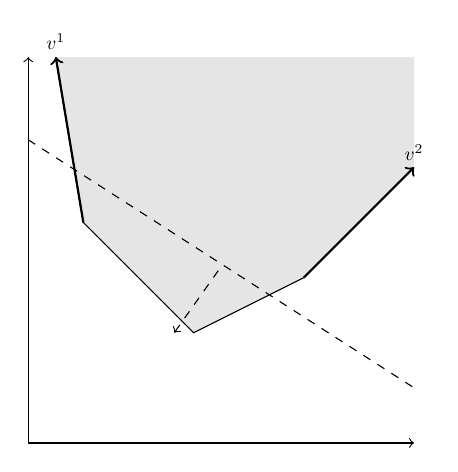
\begin{tikzpicture}[scale=.7, every node/.style = {scale = .7}]
        \draw[<->] (7, 0) -| (0, 7);
        \fill[fill=gray!20] (.5,7) -- (1,4) -- (2,3) -- (3,2) -- (5,3) -- (7,5) -- (7,7) -- cycle;
        \draw (.5,7) -- (1,4) -- (2,3) -- (3,2) -- (5,3) -- (7,5);
        \draw[->, thick] (1,4) -- (.5,7) node[above] {$v^1$};
        \draw[->, thick] (5,3) -- (7,5) node[above] {$v^2$};

        % \draw[dashed] (7,3) node[below] {$c^Tx^1$} -- (3,7);
        % \draw[dashed] (7,1) node[below] {$c^Tx^2$} -- (1,7);
        \draw[dashed] (0,5.5) -- (7, 1) ;%node[below] {$c^Tx^3$};
        % \draw[dashed] (0,4) -- (4, 0) node[below] {$c^Tx^4$};
        \draw[dashed,<-] (2.65,2) -- (3.5,3.2);

        % \draw (3.5, -1.3) node {$c^Tx^4 \ge c^Tx^3\ge c^Tx^2 \ge c^Tx^1$};
    \end{tikzpicture}
    \caption{Illustration of theorem \ref{th:upper_bounded_problem_theorem}}
    \label{fig:upper_bounded_problem}
\end{figure}

If we apply theorem \ref{th:upper_bounded_problem_theorem} to our specific problem, we find that a necessary and sufficient condition for $q(y)$ to be upper bounded is that $(b-g(y))^Tv^j\le 0, \forall j=1,...,J$ where $v^j$ denotes an extreme ray of the polyhedron $\{x|Ax\le c\}$ and $J$ a list for their indices. Moreover, we know that there exists at least one optimal solution realised in an extreme point of the feasible region. Therefore, by calling $u^i, i=1,...,I$ the extreme points of the feasible region, the problem of finding the value of $q(y)$ can be reformulated as \[ q(y) = \min\{ q : q \ge (b-g(y))^Tu^i\quad\forall i=1,...,I \} \] Assuming that this problem is bounded. We finally can write our original problem as the following
\begin{align}
    \textrm{minimize } & f(y) + q\\
    \textrm{s.t. } & y\in Y\\
    & (b-g(y))^Tu^i \le q\quad\forall i=1,...,I \label{eq:optimality_cut}\\
    & (b-g(y))^Tv^j \le 0\quad\forall j=1,...,J \label{eq:feasibility_cut}
\end{align} where constraints \ref{eq:optimality_cut} are called \textit{optimality cuts/constraints} since they define the extreme points of the feasible region and constraints \ref{eq:feasibility_cut} are called \textit{feasibility cuts/constraints} since they enforce that the problem is bounded. 

\section{Algorithm}

\subsection{Pseudo code}

It is clear that our final formulation implies an exponential number of constraints since polyhedra typically have an exponential number of extreme points and extreme rays. The idea of the Benders Decomposition Algorithm is to work with a relaxation of the problem where only a limited number of constraints are considered. The algorithm then tries to reach the optimality of the original problem by a \textit{clever} choice of constraints to be added iteratively. The algorithm is presented in \ref{alg:benders}. 
\begin{algorithm}[h!]
    \caption{Benders Decomposition Algorithm}
    \label{alg:benders}
    \begin{description}
        \item[Step 0] : Find an extreme point of $\{x|Ax\le c, x\ge 0\}$ (e.g., via the phase 1 of the Simplex)\\$1\rightarrow p, 0\rightarrow k$
        \item[Step 1] : Solve relaxed problem with only $p$ optimality constraints and $k$ feasibility constraints :
        \begin{align*}
            \textrm{minimize } & f(y) + q\\
            \textrm{s.t. } & y\in Y\\
            & (b-g(y))^Tu^i \le q\quad\forall i=1,...,p\\
            & (b-g(y))^Tv^j \le 0\quad\forall j=1,...,k
        \end{align*}
        Let $\bar y, \bar q$ be the optimal solution thus obtained. 
        \item[Step 2] : Check the feasible of $(\bar y, \bar q)$ for the original problem by solving \[ q(\bar y) = \max\{ (b-g(y))^T\pi : A^T\pi \le c, \pi\ge 0 \} \]
        Then,
        \begin{description}
            \item[If] $q(\bar y) = +\infty$ : \\
            The problem is unbounded and, from theorem \ref{th:upper_bounded_problem_theorem}, one can find an extreme ray $v^j$ such that $(b-g(y))^Tv^j > 0$. \\
            Add feasibility cut to the relaxed problem.\\
            Increment $k$. \\
            Got to \textbf{Step 1}.
            \item[Else] : \\
            Let $\bar\pi$ be the optimal solution of cost $q(\bar y)$. 
            \begin{description}
                \item[If] $\bar q < q(\bar y)$ :\\
                Add optimality cut $(b-g(y))^T\bar\pi\le q$\\
                Increment $p$.\\
                Got to \textbf{Step 1}.
                \item[Else] :\\
                The solution is optimal.
            \end{description}
        \end{description}
    \end{description}
\end{algorithm}

\subsection{Generating a feasibility cut}

In \textbf{Step 2} of algorithm \ref{alg:benders}, it is asked to find an extreme ray such that $(b-g(y))^Tv^j > 0$, i.e., a direction in which the problem is unbouned. A way to do that is to use the Simplex Tableau. Indeed, if a problem is unbounded, this implies that there exists a variable whose reduced cost is positive (i.e., ready to enter the basis) while the associated column is composed of postive terms (i.e., no constraint bounds its value). The associated column is in fact an extreme ray of the polyhedron. 

\section{Examples}

// Graphical representation

\section{Stabilisation methods}

\subsection{Bundle methods}

\subsection{Proximal methods}

\section{Generalization}

In this section, we take interest in a generalization of the Benders decomposition applicable for the following problem
\begin{align}
    \textrm{minimize } & f(x,y) \\
    \textrm{s.t. } & g(x,y) \le 0\\
    & x\in X\\
    & y\in Y
\end{align} under the following hypothesis :
\begin{enumerate}[label=($\roman*$)]
    \item $X$ is a convex set
    \item $f(x,y)$ and $g(x,y)$ are convex-in-$x$ over $X$
\end{enumerate}

It was first introduced in \cite{Geoffrion1972}. The main aspects of the demonstrations are given in this section. 

Again, we can write the \textit{projection} on the $y$-variable space, thus obtaining : 
\[
    \min\left\{ \inf\{ f(x,y) : g(x,y)\le 0, x\in X \} : y \in Y \right\}
\] where we use the convention that $\inf\{ h(x) : x\in A \} = +\infty$ if $A=\emptyset$. 

Let us denote by $v(y)$ the minimization problem over $x$, i.e., 
\[
    v(y) = \inf\{ f(x,y) : g(x,y)\le 0, x\in X \}
\] And note that $v(y)$ is considered easy to solve (by definition of $y$ as being complicating variables). Also, we will consider the following set corresponding to the feasible values of $y$ allowing one or more feasible values for $x$ : 
\[
    Y\cap V = Y\cap\left\{ y \middle| \exists x\in X, g(x, y)\le 0 \right\}
\] which turns our problem into : \[ \min\left\{ v(y) : y \in Y\cap V \right\} \] without needing any sort of convention on the infimum operator whatsoever. 

The development of the generalized Benders decomposition now depends on our ability to describe $v(y)$ and $V$, and on our ability to check the feasibility/optimality of a solution. The first two points are solved with the two following theorems :
\begin{theorem}[$V$-representation]
    Let $X$ be a non-empty convex set and $G$ be an $n$-dimensional convex-in-$x$ function for all $y\in Y$. If $\{ z\in\R^n | g(x, y)\le z \forall x\in X \}$ is closed for all $y\in Y$, then, for any $y\in Y$,
    \[ y\in V \Leftrightarrow \inf\{ \lambda^Tg(x,y) : x\in X \} \le 0, \forall\lambda\in\Lambda \]
    with $\Lambda = \left\{ \lambda\in\R^n | \sum_{i=1}^n\lambda_i = 1, \lambda \ge 0 \right\}$
\end{theorem}
\begin{proof}
\leavevmode
\begin{description}
    \item[$\Rightarrow$] : if $y\in V$ then, by definition, there exists an $x\in X$ such that $g(x,y)\le 0$ and therefore $\inf\{ \lambda^Tg(x,y) : x\in X \} \le 0, \forall\lambda\in\Lambda$. 
    \item[$\Leftarrow$] : if $\inf\{ \lambda^Tg(x,y) : x\in X \} \le 0, \forall\lambda\in\Lambda$ then \[ \sup\{ \inf\{ \lambda^Tg(x,y) \} : \lambda\in\Lambda \} \le 0 \] which implies, since the scaling of $\lambda\in\Lambda$ does not influence the sign of the quantity of which we take the supremum, that  \[ \sup\{ \inf\{ \lambda^Tg(x,y) \} : \lambda> 0 \} \le 0 \]
    And therefore, \[ \sup\{ \inf\{ \lambda^Tg(x,y) \} : \lambda\ge 0 \} = 0 \] 
    Which is equivalent to saying that the dual of the following primal problem has an optimal value of zero : 
    \begin{align*}
        \textrm{minimize } & 0^Tx\\
        \textrm{s.t. } & g(x, y) \le 0\\
        & x\in X
    \end{align*}
    The set $\{ z\in\R^n | g(x, y)\le z \forall x\in X \}$ being a closed set is a sufficient condition for the primal problem to have a feasible solution. Hence, the fact that $y\in V$
\end{description}
\end{proof}
\begin{observation}
    We give here some sufficient conditions for $\{ z\in\R^n | g(x, y)\le z \forall x\in X \}$ to be closed for any $y\in Y$ :
    \begin{itemize}
        \item $X$ is closed and bounded and $g_i(x,y)$ are continuous over $X$ for all $y\in Y$
        \item TODO
    \end{itemize}
\end{observation}

The problem can therefore be written as 
\begin{align*}
    \textrm{minimize } & h(y) \\
    \textrm{s.t. } & \inf_{x\in X}\{ \lambda^Tg(x, y) \} \le 0\quad \forall \lambda\in\Lambda\\
    & y\in Y
\end{align*}

The following theorem then reformulates problem $v(y)$ :

\begin{theorem}[$v(y)$-representation]
    Let $X$ be a non-empty convex set and assume that $f(x,y)$ and $g_i(x,y)$ are convex-in-$x$ over $X$ for any fixed $y\in Y$. Suppose also that for any $y\in Y\cap V$, the following holds :
    \begin{itemize}
        \item $h(y)$ is finite
        \item there exist optimal multipliers for the problem defining $v(y)$
    \end{itemize}
    Then, for any $y\in Y\cap V$, the primal problem defining $v(y)$ has the same optimal value as its dual :
    \[ \sup_{u\ge 0}\{ \inf_{x\in X} f(x, y) + u^Tg(x,y) \} \]
\end{theorem}
\begin{proof}
    See Lagrangian duality.
\end{proof}

The problem can now be stated, by introducing a new variable $y_0$, as
\begin{align*}
    \textrm{minimize } & y_0\\
    \textrm{s.t. } & \sup_{u\ge 0}\{ \inf_{x\in X} f(x, y) + u^Tg(x,y) \} = y_0\\
    & \inf_{x\in X}\{ \lambda^Tg(x, y) \} \le 0\quad \forall \lambda\in\Lambda\\
    & y\in Y
\end{align*}

And, by definition of the $\sup$ operator, as
\begin{align*}
    \textrm{minimize } & y_0\\
    \textrm{s.t. } & \inf_{x\in X} f(x, y) + u^Tg(x,y) \le y_0 & \forall u\ge 0\\
    & \inf_{x\in X}\{ \lambda^Tg(x, y) \} \le 0 & \forall \lambda\in\Lambda\\
    & y\in Y
\end{align*}

A simple way to solve this problem is through relaxation. We need, however, to be able to recognise situations in which the optimal solution is found or, in the contrary, to generate cuts. 

Now, note that the following so-called \textit{sub-problem} is easy to solve for a fixed value of $y = \bar y$ : 
\begin{align*}
    h(\bar y) = 
    \textrm{minimize } & f(x, \bar y)\\
    \textrm{s.t. } & g(x, \bar y) \le 0\\
    & x\in X
\end{align*}
For which three different situations can occur :
\begin{enumerate}
    \item The problem has a finite optimal value and $h(\bar y) \le y_0$ then $\bar y, y_0$ is an optimal solution of the original problem
    \item The problem has a finite optimal value and $h(\bar y) > y_0$ then, we can use an optimal vector $\bar u$ of the sub-problem and generate a new constraint 
    \[ \inf_{x\in X}\{ f(x,y) + \bar u^Tg(x,y) \le y_0 \} \]
    \item The sub-problem is not feasible, implying that $y\notin V$ and that one constraint 
    \[ \inf_{x\in X}\{ \lambda^Tg(x, y) \} \le 0 \]
    is violated for a given $\lambda$. Add the violated constraint. 
\end{enumerate}

\subsection{Pseudo-code}

We give in algorithm \ref{alg:generalized_benders}

\begin{algorithm}[h!]
    \caption{Generalized Benders Decomposition}
    \label{alg:generalized_benders}
    \begin{description}
        \item[Init] : Let $\bar y\in Y\cap V$. Find an optimal solution $\bar x$ to the sub-problem \begin{align*}
            h(\bar y) = 
            \textrm{minimize } & f(x, \bar y)\\
            \textrm{s.t. } & g(x, \bar y) \le 0\\
            & x\in X
        \end{align*} as well as an optimal multiplier $\bar u$\\
        Assign $1\rightarrow p$ and $0\rightarrow q$ and define the first relaxed problem with constraint \[ \inf_{x\in X}\{ f(x,y) + \bar u^T g(x,y) \} \le y_0 \] Also set $f(\bar x, \bar y)\rightarrow UB$ and a tolerance $\varepsilon$
        \item[Step 1] : Solve the relaxed problem 
        \begin{align*}
            \textrm{min. } & y_0\\
            \textrm{s.t. } & \inf_{x\in X}\{ f(x,y) + {u^j}^Tg(x,y) \} \le y_0 & j = 1...p\\
            & \inf_{x\in X}\{ {\lambda^j}^Tg(x,y) \} \le 0 & j = 1...q\\
            & y\in Y
        \end{align*}
        Let $\bar y,\bar y_0$ be an optimal solution to the relaxed problem. \\
        \textbf{If} $UB - \bar y_0 \le \varepsilon$, STOP. The solution is $\varepsilon$-optimal
    \end{description}
\end{algorithm}

\begin{algorithm}[h!]
    \begin{description}
        \item[Step 2] : Solve the sub-problem sub-problem \begin{align*}
            h(\bar y) = 
            \textrm{minimize } & f(x, \bar y)\\
            \textrm{s.t. } & g(x, \bar y) \le 0\\
            & x\in X
        \end{align*}
        \begin{description}
            \item[If] the sub-problem is infeasible, find $\bar\lambda\in\Lambda$ such that \[ \inf_{ x\in X }\{ \bar \lambda^Tg(x,y) \} > 0 \] Increment $q$ and introduce the constraint \[ \inf_{ x\in X }\{ \bar \lambda^Tg(x,y) \} \le 0 \] in the relaxed problem then go to \textbf{Step 1}.
            \item[Else if], there exists optimal solution to the sub-problem $\bar x$ such that $f(\bar x, \bar y) - \bar y_0 > \varepsilon$, then find an optimal multipler $\bar u$. Increment $p$ and add the following constraint to the relaxed problem :
            \[ \inf_{x\in X}\{ f(x,y) + \bar{u}^Tg(x,y) \} \le y_0 \] 
            Set $\min(UB, f(\bar x, \bar y))\rightarrow UB$, go to \textbf{Step 1}.
            \item[Else if], there exists optimal solution to the sub-problem $\bar x$ such that $f(\bar x, \bar y) - \bar y_0 \le \varepsilon$, then STOP. $\bar x, \bar y$ is a $\varepsilon$-optimal. 
        \end{description} 
    \end{description}
\end{algorithm}

\subsection{Examples}
\subsubsection{Toy bilinear problem}

\subsubsection{Two-stage Stochastic problme with recourse}